\tightsection{Evaluation}
\label{sec:eval}
We now evaluate Dante's performance and compare it with state-of-
the-art (non-FOV-aware) FEC-enabled streaming protocols as well 
as an FOV-aware TCP-based streaming protocol (DASH).
The main takeaways are two-fold. 
(1) FEC-enabled streaming protocols in general lead to higher 
PSNR than the TCP-based solution.
%, because they can work better 
%under stringent delay constraint. 
(2) By making FEC coding FOV-aware, one can further improve PSNR 
by giving FOV regions more redundancy.


\tightsubsection{Setup}

% We use a server connected with a client through a wireless link with
% controllable loss rate and latency. 
The server and client are 
commodity servers with Ubuntu 16.4 (kernel 4.40), each of which 
is equipped with an Intel(R) Core(TM) i3-4150k cpu @ 3.5GHz (4 
cores), one Intel 82599ES 10G dual port NICs and 32G memory.
They are connected with a lossy link, whose packet loss events are
generated using the Gilbert 
model ~\cite{gilbert_model}. 
Given any average packet loss rate, 
rather than dropping packets uniformly randomly, Gilbert model 
represents the network as a markovian process switching between
two states (high loss rate vs. low loss rate), and picks
the proper transition probability to match the given overall 
packet loss rate. Gilbert model is believed to be more realistic than 
uniform random packet loss~\cite{bernoulli_VS_gilbert}.
%, and uses four 
%parameters---transition probabilities between the two states and 
% the loss rate of each state---to control the overall packet loss 
% rate. So the Gilbert model is believed to be more realistic than 
% uniform random packet loss~\cite{bernoulli_VS_gilbert}. 
We use Gilbert model to generate two 
network traces: one for ``good'' network condition (loss rate $=0.5\%$), and one for
``bad'' network condition (loss rate $=2\%$). 
Table~\ref{tab:parameters} shows the
parameter settings of each trace. 
We use Linux TC~\cite{TC} to control the actual instantaneous loss rate. 

\begin{table}[t]
	\centering 
	\scriptsize
	\begin{tabular}{cp{1.0cm}p{1.6cm}p{0.8cm}p{2.3cm}}
		\rowcolor[gray]{0.9} 
		\hline
		(A)  &  Time(Sec.)    & network capacity(Mbps)       &  RTT(ms) &  Average Pakcet loss rate(\%) \\

		
		&  0${\sim}$60   &  30         &    50    &  0.5 \\

		\hline
		\rowcolor[gray]{0.9}
		\hline
		(B)  &   Time(Sec.)   & Bandwidth(Mbps)       &  RTT(ms) &     Average Pakcet loss rate(\%)  \\
		
		&  0${\sim}$60   &  20         &    50    &  2.0\\
		
		\hline
		
	\end{tabular}
	\vspace{0.5cm}
	\tightcaption{Network Condition of Two Wireless networks: (A)Relatively Good Wireless Conditions And (B)Relatively Bad Wireless Conditions}
	\vspace{-0.3cm}
	\label{tab:parameters}
\end{table}



\begin{figure*}[!t]
	%\begin{figure*}[t]
	\centering
    % \subfigure[Video Sequence 1]  {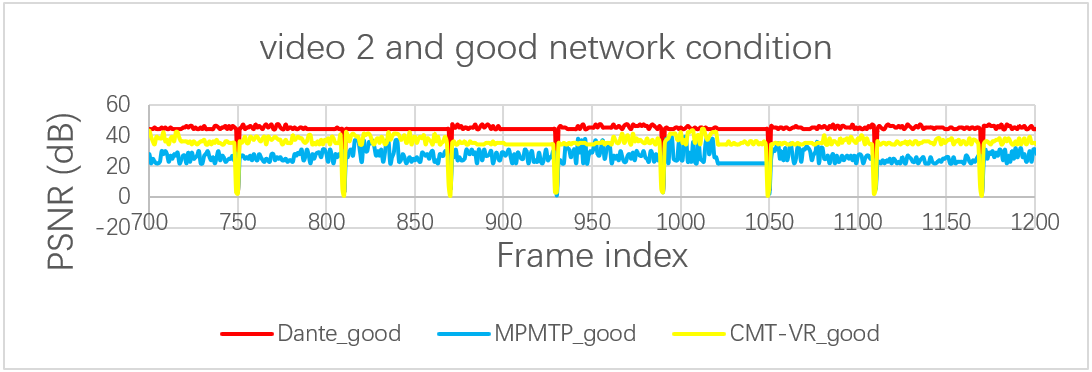
\includegraphics[scale=0.26,angle=0]{paper_figs/evaluation_result/sub/ins_psnr_v2_good.png}}
    % \subfigure[Video Sequence 2]  {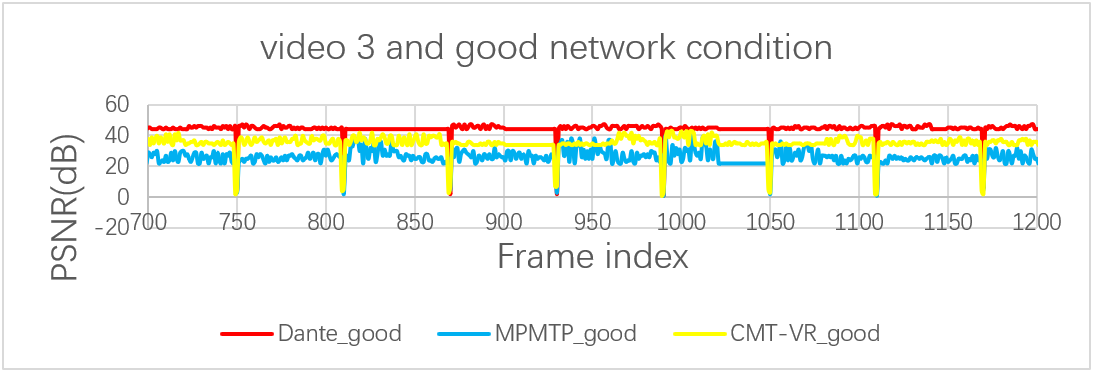
\includegraphics[scale=0.26,angle=0]{paper_figs/evaluation_result/sub/ins_psnr_v3_good.png}}
    \subfigure[Video \#1]  {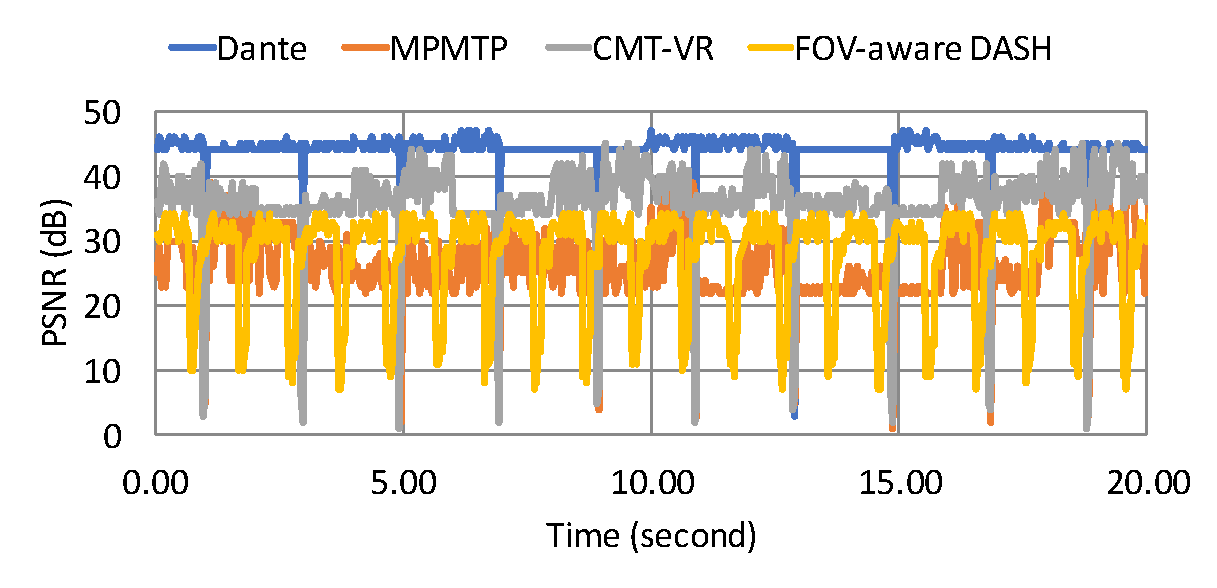
\includegraphics[width=0.4\textwidth]{paper_figs/dante-good-video-1.pdf}}
    % \hspace{-0.3cm}
	\subfigure[Video \#2]  {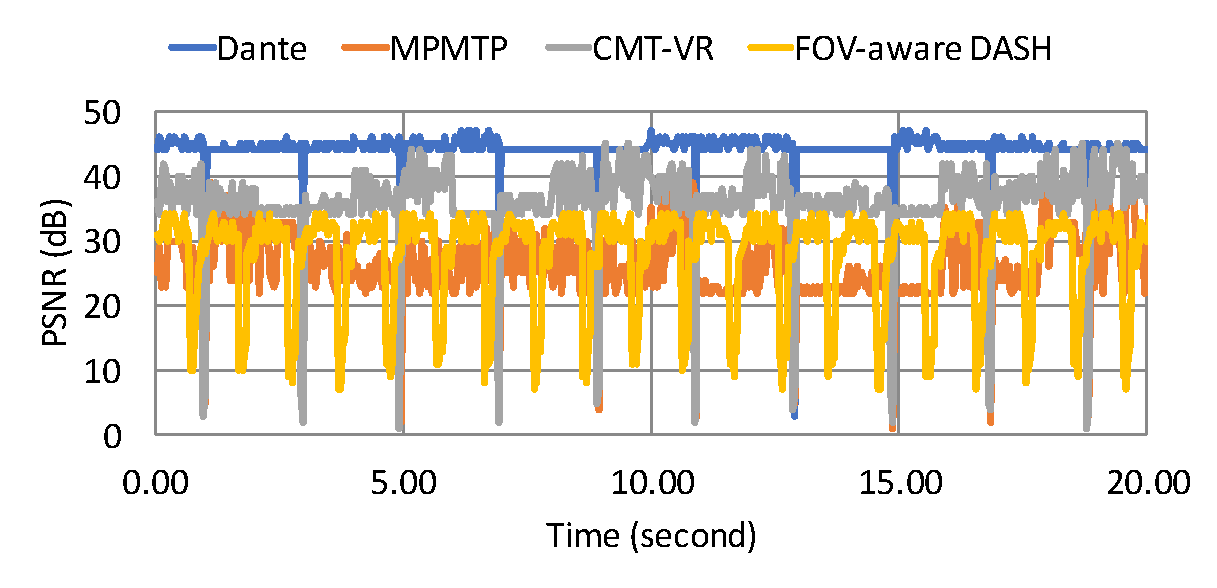
\includegraphics[width=0.4\textwidth]{paper_figs/dante-good-video-2.pdf}}
% 	\vspace{-0.3cm}
	\tightcaption{Dante outperforms three baselines under the relatively good network condition (avg. packet loss rate $=0.5\%$).}
	\vspace{-0.6cm}
	\label{fig:good}
\end{figure*}

%*****Instantaneous PSNR In relatively Good Network Condition*****
\begin{figure*}[!t]
	%\begin{figure*}[t]
	\centering
% 	\subfigure[Video Sequence 1]  {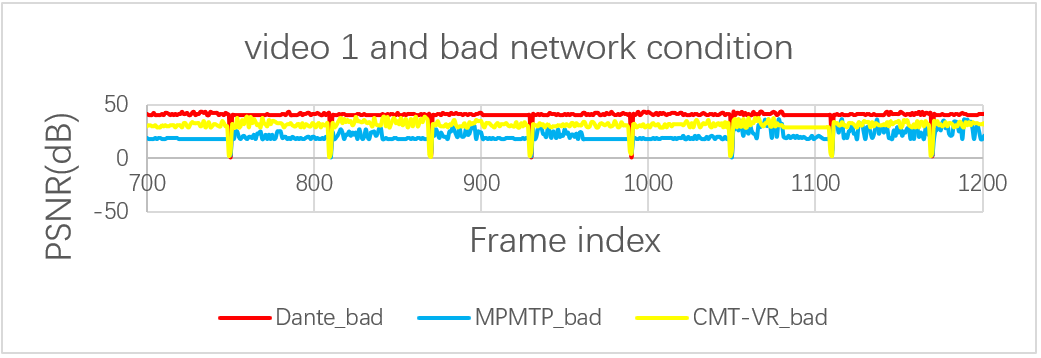
\includegraphics[scale=0.275,angle=0]{paper_figs/evaluation_result/sub/ins_psnr_v1_bad.png}}
% 	\subfigure[Video Sequence 2]  {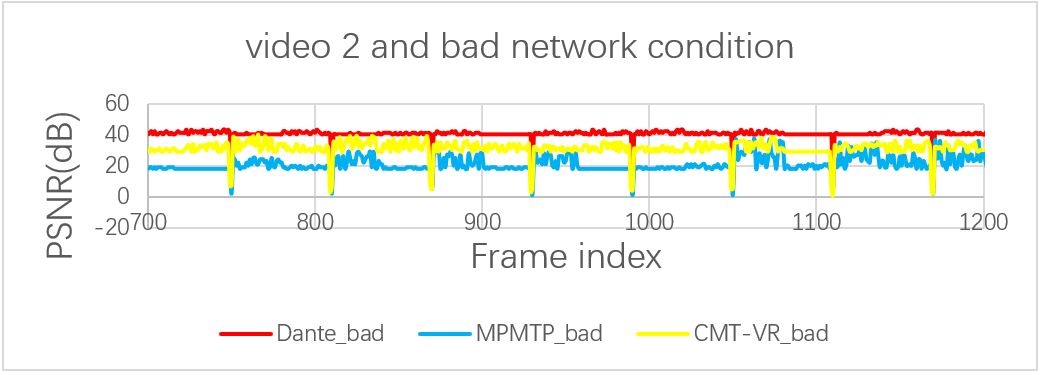
\includegraphics[scale=0.27,angle=0]{paper_figs/evaluation_result/sub/ins_psnr_v2_bad.png}}
    \subfigure[Video \#1]  {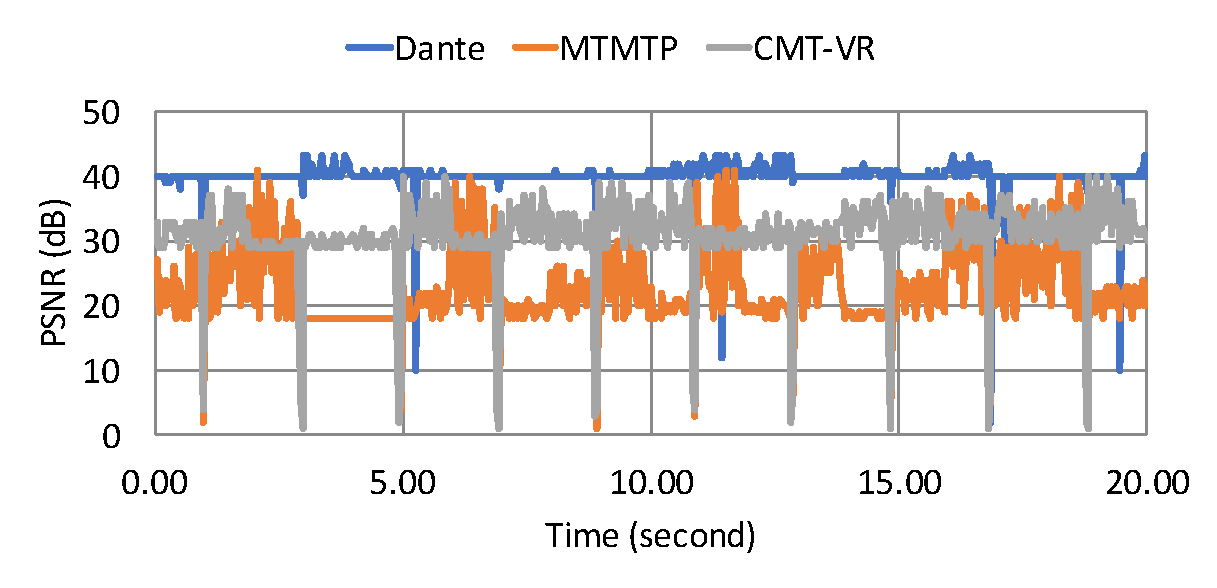
\includegraphics[width=0.4\textwidth]{paper_figs/dante-bad-video-1.pdf}}
    % \hspace{-0.3cm}
	\subfigure[Video \#2]  {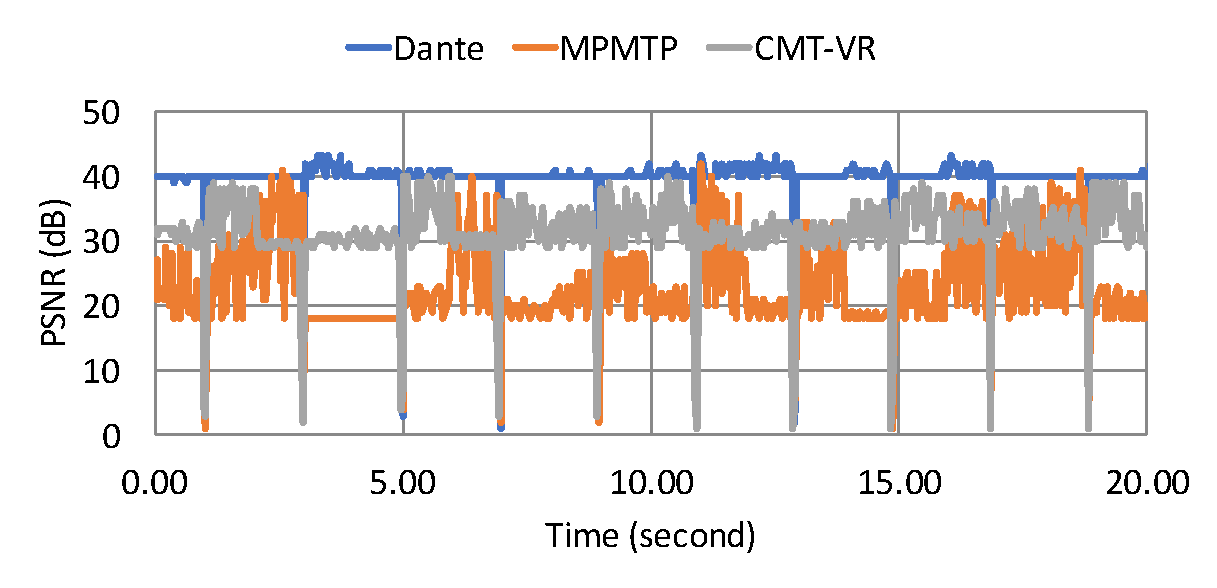
\includegraphics[width=0.4\textwidth]{paper_figs/dante-bad-video-2.pdf}}
% 	\vspace{-0.3cm}
	\tightcaption{Dante outperforms three baselines under the relatively bad network condition (average packet loss rate of 2\%). DASH is not shown here since TCP performs badly under such network condition.}
	\vspace{-0.2cm}
	\label{fig:bad}
\end{figure*}

We use two 360-degree video sequences downloaded from Youtube, 
each of 60 seconds and encoded in H.265 format with a frame rate of 30 frames per second and a GOP size 
of 15 frames. Each frame is split into 72 uniformly 
sized tiles, and we assume users will watch the FOV-region tiles 
(15\% of all tiles) with 60\% probability, cushion-region tiles 
(25\% of all tiles) with 30\% probability, FOV-region tiles (60\% 
of all tiles) with 10\% probability. These settings are aligned 
with prior work (\eg~\cite{360ProbDASH}). Based on this probability 
distribution, we measure the overall quality by the sum 
of PSNR value of each tile weighted by the probability of them 
being watched.

We compare Dante with three baselines:
\begin{packeditemize}

\item {\em FOV-aware DASH}~\cite{Omnidirectional_Video_over_HTTP} 
is built on HTTP/TCP and uses an FOV-aware tile-based streaming 
scheme to reduce bandwidth consumption.

\item {\em MPMTP}~\cite{MPMTP} uses the FEC to recover the data 
without any retransmission. It treats all frames 
separately and thus ignores the interdependency between frames. 

\item {\em CMT-VR}~\cite{CMT-VR} uses quality-driven FEC 
redundancy allocation to minimize the distortion of each GOP and 
Raptor code to avoid retransmission. Unlike MPMTP, it considers 
inter-frame dependency. Both CMT-VR and MPMTP are not FOV-aware. 

\end{packeditemize}




\tightsubsection{Preliminary results}



Then, Figure \ref{fig:good} and Figure \ref{fig:bad} compare instantaneous PSNR of two video sequences in good network condition and bad network condition, respectively. These result show that Dante achieves 20\% to 30\% 360-degree video PSNR performance gain, compared to MPMTP and CMT-VR and 40\% PSNR performance gain, compared to FOV-aware DASH. DASH performs worst since it's underlying TCP protocol achieves poor throughput in high lossy networks. 
The reason why MPMTP also performs badly among these protocols is that, despite maximizing the throughput without any retransmission, it doesn't make extra effort to guarantee the reliability of I frames. So, once I frames can not be recovered from burst packet loss, the GOP of video even can not be normally decoded by video codec and thus resulting in poor performance. Meanwhile, CMT-VR performs better than MPMTP, mainly due to its consideration of frame priority. However, unfortunately, it's non-FOV-aware reliability scheme makes itself waste too much bandwidth on trivial data. Dante takes into account not only traditional video features, like frame priority, but FOV, meanwhile. Benefiting from the hierarchical protection spatially and temporally, Dante achieves desirable upgrade in instantaneous PSNR. Meanwhile, we find, compared to TCP without FEC, the average CPU time of Dante's cients, considering the average CPU time of socket, FEC decoding, video codec as well as rendering, increase from 113\% to 126\%. The almost 11.5 percentage of the extra cpu overhead of FEC can be ignored considering the performance gain Dante achieves.    